% Full instructions available at:
% https://github.com/elauksap/focus-beamertheme

\documentclass{beamer}
\usetheme[numbering=progressbar]{focus}
\usepackage{tikz}
\usetikzlibrary{positioning}
\usetikzlibrary{shapes,arrows}
\usepackage{transparent}
\usepackage{fancyvrb}
\usepackage{listings}
\usepackage{tabularx}
\usepackage{amsfonts}
\usepackage{ulem}
\usepackage{csquotes}
\definecolor{main}{RGB}{47, 161, 219}
\definecolor{background}{RGB}{240, 247, 255}
\definecolor{textcolor}{RGB}{85, 87, 83}

\title{Mind your Ps and Qs: }
\subtitle{Performing crypto sanity checks with D4.}
\author{Jean-Louis Huynen}
\titlegraphic{
\includegraphics[scale=0.20]{../../logos/d4-logo.pdf}}
\institute{Team CIRCL \\ \url{https://www.d4-project.org/}}
\date{November 12, 2019}

\begin{document}
    \begin{frame}
        \maketitle
    \end{frame}

\begin{frame}
        \frametitle{D4 - Problem statement}
        \begin{itemize}
                \item CSIRTs (or private organisations) build their {\bf own honeypot, honeynet or blackhole monitoring network}
                \item Designing, managing and operating such infrastructure is a tedious and resource intensive task
                \item {\bf Automatic sharing} between monitoring networks from different organisations is missing
                \item Sensors and processing are often seen as blackbox or difficult to audit

        \end{itemize}
\end{frame}


\begin{frame}
 \frametitle{D4 - Objective}
 \begin{itemize}
         \item Based on our experience with
           MISP\footnote{\url{https://github.com/MISP/MISP}} where sharing
           played an important role, we transpose the model in D4 project
         \item Keeping the protocol and code base {\bf simple and minimal}
         \item Allowing every organisation to {\bf control and audit their own sensor network}
         \item Extending D4 or {\bf encapsulating legacy monitoring protocols} must be as simple as possible
         \item Ensuring that the sensor server has {\bf no control on the sensor} (unidirectional streaming)
         \item Don't force users to use dedicated sensors and allow {\bf flexibility of sensor support} (software, hardware, virtual)

 \end{itemize}
\end{frame}

\begin{frame}
        \frametitle{D4 - (short) History}
 \begin{itemize}
        \item D4 Project (co-funded under INEA CEF EU program) started - {\bf 1st November 2018}
        \item D4 encapsulation protocol version 1 published  - {\bf 1st December 2018}
        \item v0.1 release of the D4 core\footnote{\url{https://www.github.com/D4-project/d4-core}} including a server and simple D4 C client - {\bf 21st January 2019}
        \item First version of a golang D4
          client\footnote{\url{https://www.github.com/D4-project/d4-goclient/}}
          running on ARM, MIPS, PPC and x86 - {\bf 14th February 2019}
 \end{itemize}
\end{frame}

\begin{frame}
\frametitle{D4 - Overview}
        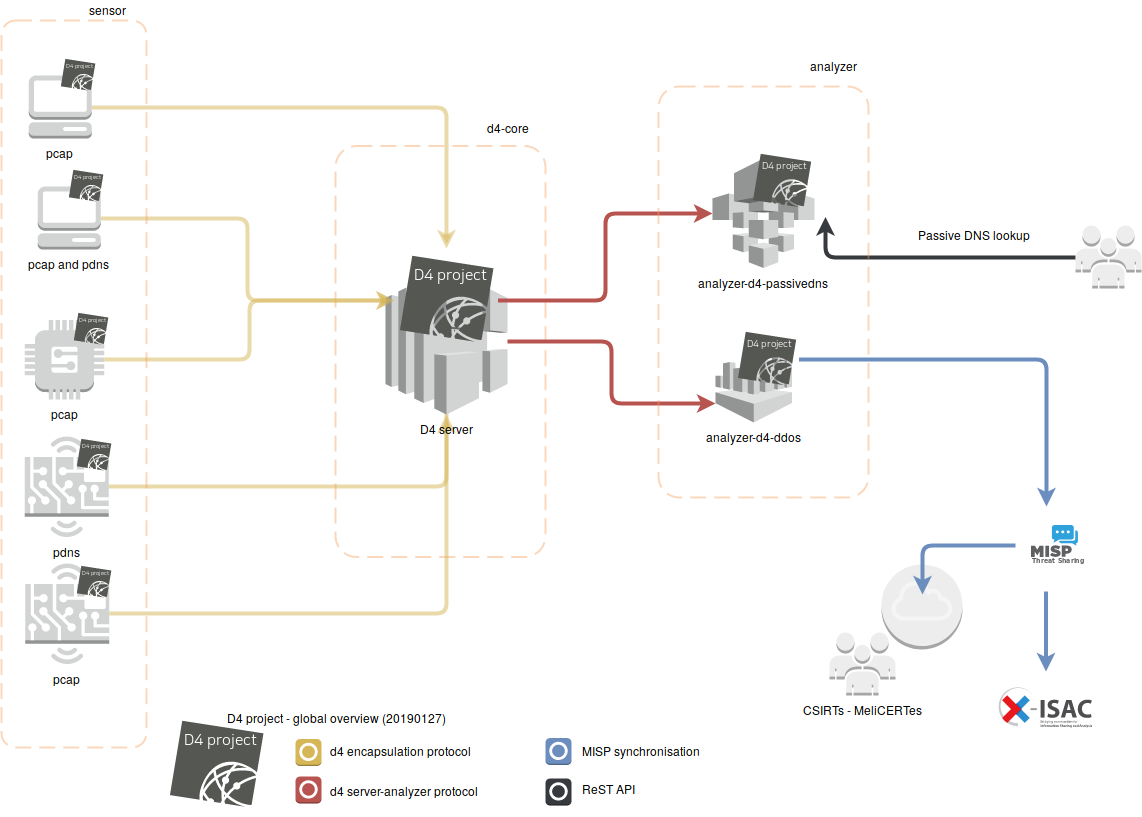
\includegraphics[scale=0.38]{../../diagram/d4-overview.png}
\end{frame}


\begin{frame}
  \frametitle{Snake Oil Crypto - Problem Statement}
  IoT devices {\bf are often the weakest devices} on a network:
        \begin{itemize}
        \item Usually the result of cheap engineering,
        \item sloppy patching cycles,
        \item sometimes forgotten--not monitored,
        \item few hardening features enabled,
        \end{itemize}

        \vspace{10 mm} 

{\bf We feel a bit safer when they use TLS, but should we?}

\end{frame}

\begin{frame}
  \frametitle{Snake Oil Crypto - TLS Fingerprinting}
        {\bf Keep} a log of links between:
        \begin{itemize}
          \item x509 certificates,
          \item ports,
          \item IP address,
          \item client (ja3),
          \item server (ja3s),
        \end{itemize}
        \begin{displayquote}
        ``JA3 is a method for creating SSL/TLS client fingerprints that should be easy to produce on any platform and can be easily shared for threat intelligence.''\footnote{https://github.com/salesforce/ja3}
        \end{displayquote}

         {\bf Pivot} on additional data points during Incident Response 
\end{frame}

\begin{frame}
   \frametitle{Snake Oil Crypto -  Objectives}
   {\bf Collect} and {\bf store} x509 certificates and TLS sessions:
        \begin{itemize}
        \item Public keys type and size,
        \item moduli and public exponents,
        \item curves parameters.
        \end{itemize}
        {\bf Detect} anti patterns in crypto:
        \begin{itemize}
          \item Moduli that share one prime factor,
          \item Moduli that share both prime factors, or private exponents,
          \item Small factors,
          \item Nonces reuse / common preffix or suffix, etc. 
        \end{itemize}
\end{frame}


\begin{frame}[fragile]
   \frametitle{Snake Oil Crypto - RSA on IoT }
   Researchers have shown that several devices generated their public
   keys at boot time without enough entropy\footnote{Bernstein, Heninger, and Lange: \url{http://facthacks.cr.yp.to/}}:
   
\begin{lstlisting}[frame=single, language=python]
prng.seed(seed)
p = prng.generate_random_prime()
// prng.add_entropy()
q = prng.generate_random_prime()
n = p*q
\end{lstlisting}

Given n=pq and n' = pq' it is trivial to recover the shared p by computing their
Greatest Common Divisor (GCD), and therefore both private keys\footnote{\url{http://www.loyalty.org/~schoen/rsa/}}.

\end{frame}

\begin{frame}
   \frametitle{Snake Oil Crypto - GCD}
   In Snake-Oil-Crypto we compute GCD\footnote{using Bernstein's Batch GCD algorithm} between:
   
   \begin{itemize}
     \item between certificates having the same issuer,
     \item between certificates having the same subject,
     \item on keys from various sources (PassiveSSL, Certificate Transparency,
       shodan, censys, etc.),
   \end{itemize}

\vspace{10 mm}
  {\bf ``Check all the keys that we know of for vendor X''}

\end{frame}

\begin{frame}
   \frametitle{Snake Oil Crypto - MISP feed}
\begin{figure}
\centering
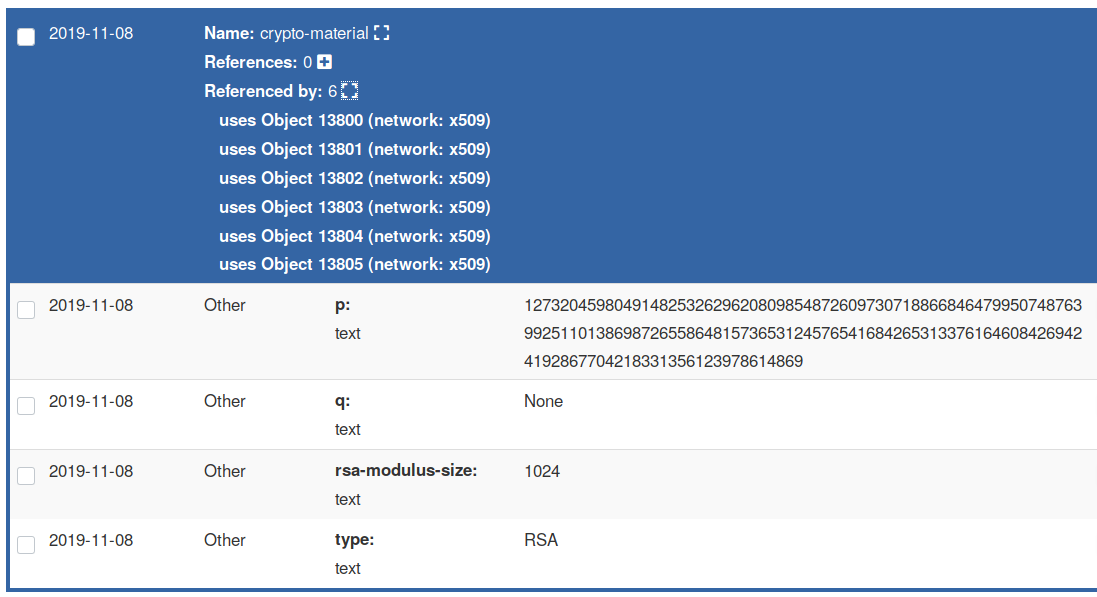
\includegraphics[width=\textwidth]{misp.png}
\end{figure}

\end{frame}

\begin{frame}
   \frametitle{Snake Oil Crypto - MISP feed}
   The MISP feed
   \begin{itemize}
     \item {\bf Allows} for checking automatic checking by an IDS on hashed values,
     \item {\bf contains} thousands on broken keys from a dozen of vendors,
     \item {\bf will be accessible upon request (info@circl.lu).}
   \end{itemize}

   In the future:
    \begin{itemize}
     \item {\bf Automatic} the vendor checks by performing TF-IDF on x509's subjects, 
     \item {\bf automatic} vendors notification.
     \end{itemize}

\end{frame}


\begin{frame}
  \frametitle{First release}
  \begin{itemize}
  \item[\checkmark] sensor-d4-tls-fingerprinting
    \footnote{\url{github.com/D4-project/sensor-d4-tls-fingerprinting}}:
    {\bf Extracts} and {\bf fingerprints} certificates, and {\bf computes} TLSH fuzzy hash.
  \item[\checkmark] analyzer-d4-passivessl
    \footnote{\url{github.com/D4-project/analyzer-d4-passivessl}}:
    {\bf Stores} Certificates / PK details in a PostgreSQL DB.
  \item snake-oil-crypto 
    \footnote{\url{github.com/D4-project/snake-oil-crypto}}:
    {\bf Performs} crypto checks, push results in MISP for notification
  \item lookup-d4-passivessl
    \footnote{\url{github.com/D4-project/lookup-d4-passivessl}}:
    {\bf Exposes} the DB through a public REST API.
  \end{itemize}
\end{frame}

\begin{frame}
\frametitle{Use it}
\begin{itemize}
\item {\bf Manage} your own sensors and servers, {\bf find} shameful bugs and
  {\bf fill} in github issues
\item Even better, {\bf send} Pull Requests! 
\item {\bf Share} data to public servers to improve the datasets (and detection,
  response, etc.)
\item {\bf Feed} your MISP instances with D4's findings - {\bf Share} yours
\item {\bf Leech} data, {\bf write} your own analyzers, {\bf do} research
\end{itemize}
\end{frame}

\begin{frame}
\frametitle{Get in touch if you want to join the project, host a sensor or contribute}
\begin{itemize}
\item Collaboration can include research partnership, sharing of collected streams or improving the software.
\item Contact: info@circl.lu
\item \url{https://github.com/D4-Project}
\item \url{https://twitter.com/d4_project}
\item \url{https://d4-project.org}
\begin{itemize}
  \item
    \href{https://d4-project.org/2019/05/28/passive-dns-tutorial.html}{Passive DNS tutorial}
  \item
    \href{https://d4-project.org/2019/06/17/sharing-between-D4-sensors.html}{Data
      sharing tutorial}
\end{itemize}
\end{itemize}
\end{frame}


\end{document}
